\frame{\tableofcontents[currentsection]}

\subsection{Motivation: The Grothendieck-Tsirelson Theorem}
\frame{\tableofcontents[currentsubsection]}
	\begin{frame}
		\begin{theo}[Grothendieck-Tsirelson]
			There exists an absolute constant $K\geq 1$ such that, for any positive integers $m,n$, the following three equivalent conditions hold:
			\begin{itemize}
				\item[(1)] We have the inclusion 
					\begin{equation}
						\QC_{m,n} \subset K\LC_{m,n}.
					\end{equation}
				\item[(2)] For any $M\in\mathbb{R}^{m\times n}$ and for any $\rho,X_i,Y_j$ verifying the conditions of Definition \textcolor{red}{4.2.1} we have
					\begin{align}
						\sum_{i,j} M_{ij} \trace{\rho(X_i\tensor Y_j)} &\leq K \max_{\xi\in\{-1,1\}^m,\eta\in\{-1,1\}^n} \sum_{i,j} M_{ij}\xi_i\eta_j \\
						\Leftrightarrow \hspace{2.5cm} \trace{MA^\top} &\leq \max_{\xi\in\{-1,1\}^m,\eta\in\{-1,1\}^n} \trace{M(\xi\eta^\top)^\top}.
					\end{align}
					\item[(3)] For any $M\in\mathbb{R}^{m\times n}$ and for any (real) Hilbert space vectors $x_i,y_j$ with $\modul{x_i}\leq 1$, $\modul{y_j}\leq 1$ we have
						\begin{equation}
							\sum_{i,j} M_{i,j}\sclr{x_i}{y_j} \leq K \max_{\xi\in\{-1,1\}^m,\eta\in\{-1,1\}^n} \trace{\xi^\top M \eta}. \label{eq:G_ineq}
						\end{equation}
			\end{itemize}
		\end{theo}
	\end{frame}

\subsection{Grothendieck's Inequality}
	\frame{\tableofcontents[currentsubsection]}
	\begin{frame}
		\begin{lemma}[Grothendieck's identity]\label{lem:G_id}
			Let $x,y\in S^{d-1}$. Let $r\in S^{d-1}$ be a random unit vector chosen from $O(d)$-invariant probability distribution on the unit sphere. Then
			\begin{enumerate}
				\item[i,] $\mathbb{P}[\sgn(\sclr{x}{r})\neq\sgn(\sclr{y}{r})]=\frac{\arccos(\sclr{x}{y})}{\pi}$
				\item[ii,] $\mathbb{E}[\sgn(\sclr{x}{r})\sgn(\sclr{y}{r})]=\frac{2}{\pi}\arcsin(\sclr{x}{y}).$
			\end{enumerate}
		\end{lemma}
		\begin{pbmr}
			\begin{itemize}
				\item<1-> If $x$ and $y$ are linearly dependent, then
					\begin{itemize}
						\item<2-> if $x=y$:~~\, $\arccos(\sclr{x}{y})=\arccos(1) = 0$.
						\item<3-> if $x=-y$: $\arccos(\sclr{x}{y})=\arccos(-1) = \pi$.
					\end{itemize}
				\item<4-> If $x$ and $y$ are linearly independent, then 
					\begin{itemize}
						\item<5-> project $r$ orthogonally on $\spn\{x,y\}$ which gives us a vector $s$ with $\sclr{x}{r} = \sclr{x}{s}$ and $\sclr{y}{r} = \sclr{y}{s}$,
						\item<6-> the normalized vector $n\coloneqq s/\modul{s}$ is uniformly distributed on the intersection of the unit sphere and $\spn\{x,y\}$ by the $O(d)$-invariance of the probability distribution.
	%					\item<7-> $\mathbb{P}[\sgn(\sclr{x}{r})\neq\sgn(\sclr{y}{r})]= \mathbb{P}[\sgn(\sclr{x}{n})\neq\sgn(\sclr{y}{n})]$, where $n\coloneqq s/\modul{s}$ by the $O(d)$-invariance of the probability distribution
					\end{itemize}
			\end{itemize}
		\end{pbmr}
	\end{frame}
	
	\begin{frame}
		\begin{pbmr}[Proof (cont.).]
			Calculation of the probability that the signs of the scalar products $\sclr{x}{n}$ and $\sclr{y}{n}$ are unlike:
			\begin{figure}
				\begin{center}
					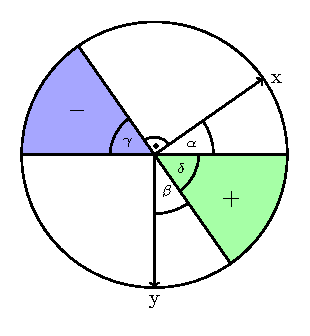
\includegraphics[width=0.38\textwidth]{ChapersPresentation/fig_unit_circle.pdf}
				\end{center}
				\vspace{-2em}
			\end{figure}
			\begin{align*}
				\mathbb{P}[\sgn(\sclr{x}{n})\neq\sgn(\sclr{y}{n})]=2\frac{\arccos(\sclr{x}{y})}{2\pi} = \frac{\arccos(\sclr{x}{y})}{\pi}
			\end{align*}
		\end{pbmr}
	\end{frame}
	
	\begin{frame}
		\begin{proof}[Proof (cont.).]
			We conclude with the proof of the second part of Lemma \ref{lem:G_id}: 
			\begin{align*}
				&\mathbb{E}[\sgn(\sclr{x}{r}) \sgn(\sclr{y}{r})] \\
				&\qquad= 1 - 2 \frac{\arccos(\sclr{x}{y})}{\pi} \\
				&\qquad= \frac{2}{\pi} \arcsin(\sclr{x}{y}),
			\end{align*}
			because $\arcsin (t) + \arccos(t) = \pi/2$.
		\end{proof}
	\end{frame}
	\begin{frame}
		\begin{lemma}[Krivine's trick]\label{lem:krivines_trick}
			Let $x_1,\dots,x_m,y_1,\dots,y_n\in S^{m+n-1}$ be given. Furthermore, let $r\in S^{n+m-1}$ be a random unit vector chosen form the $O(n+m-1)$-invariant probability distribution on the unit sphere. Then there are $x_1^\prime,\dots,x_m^\prime, y_1^\prime,\dots,y_n^\prime\in S^{m+n-1}$ so that
			\begin{equation}
				\mathbb{E}[\sgn(\sclr{x_i^\prime}{r})\sgn(\sclr{y_j^\prime}{r})] = \beta \sclr{x_i}{y_j},
				\label{eq:krivines_trick}
			\end{equation}		
			with $\beta = \frac{2}{\pi} \ln (1+\sqrt{2}).$
		\end{lemma}
	\end{frame}
	\begin{frame}
		\begin{definition}[The $k$-th tensor product]
			The \emph{$k$-th tensor product} of $\mathbb{R}^n$ with orthonormal basis $e_1,\dots,e_n$ is denoted by $(\mathbb{R}^n)^{\tensor k}$ and it is a Euclidean vector space of dimension $n^k$ with othonormal basis $e_{i_1}\tensor \cdots \tensor e_{i_k}$, $i_l\in\{1,\dots,n\}$. In particular 
			\begin{align}
				\sclr{e_{i_1}\tensor \cdots \tensor e_{i_k}}{e_{j_1}\tensor \cdots \tensor e_{j_k}}
			&= \prod_{l=1}^k \sclr{e_{i_l}}{e_{j_l}}\nonumber\\
			&=\begin{cases}
				1 & , \text{ if } i_l=j_l \text{ for all } l=1,\dots,n,\\
				0 & , \text{ otherwise},
			\end{cases} \label{eq:orthonormtensor}
			\end{align}
			and for $v\in\mathbb{R}^n$ with $v=v_1e_1+\cdots +v_ne_n$ we define $v^{\tensor k} \in (\mathbb{R}^n)^{\tensor k}$ by 
			\begin{align}
				v^{\tensor k} &\coloneqq (v_1e_1 + \cdots + v_ne_n) \tensor \cdots \tensor (v_1e_1 + \cdots + v_ne_n) \nonumber\\
				&= \sum_{i_1,\dots,i_k} v_{i_1}\cdots v_{i_k} e_{i_1}\tensor\cdots\tensor e_{i_k}.
			\end{align}	
		\end{definition}
		Thus, for $v,w\in\mathbb{R}^n$ 
		\begin{align}
			\sclr{v^{\tensor k}}{w^{\tensor k}}
			= \sclr{v}{w}^k. \label{eq:kth_tensor}
		\end{align}
	\end{frame}
	\begin{frame}
		\begin{lemma}[Krivine's trick]\label{lem:krivines_trick}
			Let $x_1,\dots,x_m,y_1,\dots,y_n\in S^{m+n-1}$ be given. Furthermore, let $r\in S^{n+m-1}$ be a random unit vector chosen form the $O(n+m-1)$-invariant probability distribution on the unit sphere. Then there are $x_1^\prime,\dots,x_m^\prime, y_1^\prime,\dots,y_n^\prime\in S^{m+n-1}$ so that
			\begin{equation}
				\mathbb{E}[\sgn(\sclr{x_i^\prime}{r})\sgn(\sclr{y_j^\prime}{r})] = \beta \sclr{x_i}{y_j},
				\label{eq:krivines_trick}
			\end{equation}		
			with $\beta = \frac{2}{\pi} \ln (1+\sqrt{2}).$
		\end{lemma}
		\begin{pbmr}[Proof of Krivine's trick.]
			\begin{itemize}
				\item<1-> Define $E: [-1,+1] \to [-1,+1]$ by $E(t)=\frac{2}{\pi}\arcsin(t)$.
				\item<2-> $E(\sclr{x_i^\prime}{y_j^\prime} ) = \mathbb{E}[\sgn(\sclr{x_i^\prime}{r})\sgn(\sclr{y_j^\prime}{r})] \overset{!}{=}\beta \sclr{x_i}{y_j}$ by Grothendieck's identity.
				\item<3-> Idea: To find $\beta,x_i^\prime,y_j^\prime$ invert $E$:  
					\[
						E^{-1}(t) = \sin(\pi/2 \cdot t) 
						= \sum_{k=0}^\infty \underbrace{\frac{(-1)^{2k+1}}{(2k+1)!}\left(\frac{\pi}{2}\right)^{2k+1}}_{\eqqcolon g_{2k+1}}  t^{2k+1},
					\]
%					such that $\sclr{x_i^\prime}{y_j^\prime} = E^{-1}(\beta\sclr{x_i}{y_j})$ 
			\end{itemize}
		\end{pbmr}
	\end{frame}
	\begin{frame}
		\begin{pbmr}[Proof (cont.).]
			\begin{itemize}
				\item<1-> Define the infinite-dimensional Hilbert space
					\begin{equation}
						H= \bigoplus_{r=0}^\infty (\mathbb{R}^{m+n})^{\tensor 2k+1}.
					\end{equation}
				\item<2-> Define $\tilde{x}_i, \tilde{y}_j\in H$, $i=1,\dots,m,j=1,\dots,n$ componentwise:
					\begin{align}
						(\tilde{x}_i)_k &= \sgn(g_{2k+1}) \sqrt{\modul{g_{2k+1}}\beta^{2k+1}}\, x_i^{\tensor 2k+1} \\
						(\tilde{y}_j)_k &= \sqrt{\modul{g_{2k+1}}\beta^{2k+1}} \,y_j^{\tensor 2k+1}
					\end{align}
				\item<3-> Then
					\begin{align*}
						\sclr{\tilde{x}_i}{\tilde{y}_j} &= \sum_{k=0}^\infty g_{2k+1} \beta^{2k+1}\sclr{x_i^{\tensor 2k+1}}{y_j^{\tensor 2k+1}} \\
						&= \sum_{k=0}^\infty g_{2k+1} \beta^{2k+1} \sclr{x_i}{y_j}^{2k+1} \\
						&= E^{-1}(\beta \sclr{x_i}{y_j}).
					\end{align*}
			\end{itemize}
		\end{pbmr}
	\end{frame}
	\begin{frame}
		\begin{pbmr}[Proof (cont.).]
			\begin{itemize}
				\item<1-> Hence, $\beta$ is defined by the condition that the vectors $\tilde{x}_1,\dots,\tilde{x}_m,\tilde{y}_1,\dots,\tilde{y}_n$ are unit vectors:
					\begin{gather*}
						1 = \sclr{\tilde{x}_i}{\tilde{x}_i} = \sclr{\tilde{y}_j}{\tilde{y}_j}
						= \sum_{k=0}^\infty \frac{1}{(2k+1)!}\left(\frac{\pi}{2}\right)^{2k+1}\beta^{2k+1}=\sinh(\frac{\pi}{2}\beta)\\
						\Leftrightarrow \qquad\beta = \frac{2}{\pi} \arcsinh(1) = \frac{2}{\pi}\ln(1+\sqrt{2}) \qquad\quad~
					\end{gather*}
				\item<2-> Problem: $\tilde{x}_1,\dots,\tilde{x}_m,\tilde{y}_1,\dots,\tilde{y}_n$ are infinite-dimensional
				\item<3-> Solution: the positive definite and symmetric Gram matrix $G$
					\begin{equation}
						G=\begin{pmatrix}
							\sclr{\tilde{x}_1}{\tilde{x}_1} & \cdots & \sclr{\tilde{x}_1}{\tilde{x}_m}& \sclr{\tilde{x}_1}{\tilde{y}_1} & \cdots & \sclr{\tilde{x}_1}{\tilde{y}_n} \\
							 \vdots		& \ddots	& \vdots & \vdots & \ddots & \vdots\\
							 \sclr{\tilde{x}_m}{\tilde{x}_1} & \cdots & \sclr{\tilde{x}_m}{\tilde{x}_m}& \sclr{\tilde{x}_m}{\tilde{y}_1} & \cdots & \sclr{\tilde{x}_m}{\tilde{y}_n} \\
							\sclr{\tilde{y}_1}{\tilde{x}_1} & \cdots & \sclr{\tilde{y}_1}{\tilde{x}_m}& \sclr{\tilde{y}_1}{\tilde{y}_1} & \cdots & \sclr{\tilde{y}_1}{\tilde{y}_n} \\
							 \vdots		& \ddots	& \vdots& \vdots & \ddots & \vdots\\
							 \sclr{\tilde{y}_n}{\tilde{x}_1} & \cdots & \sclr{\tilde{y}_n}{\tilde{x}_m}& \sclr{\tilde{y}_n}{\tilde{y}_1} & \cdots & \sclr{\tilde{y}_n}{\tilde{y}_n} 
						\end{pmatrix}
					\end{equation}
			\end{itemize}
		\end{pbmr}
	\end{frame}
	
	\begin{frame}
		\begin{proof}[Proof (cont.).]
			\begin{itemize}
				\item<1-> Due to the properties of $G$ we can decompose $G$ via a real orthogonal matrix $Q$ with columns that are the eigenvectors of $G$ and a real diagonal matrix $\Lambda$ having the eigenvalues of $G$ on the diagonal, thus
					\begin{equation}
						G=Q\Lambda Q^\top =(\underbrace{Q\Lambda^{1/2}}_{\eqqcolon A})^\top(Q\Lambda^{1/2}).
					\end{equation}
				\item<2-> The columns of $A$ are the vectors $x_1^\prime,\dots,x_m^\prime,y_1^\prime,\dots,y_n^\prime \in S^{m+n-1}$ we are looking for.
			\end{itemize}
		\end{proof}
	\end{frame}
	
	\begin{frame}
		\begin{dfn}
			For $M\in\mathbb{R}^{m\times n}$ define the quadratic program
			\begin{align}
				\norm{M}_{\infty\to 1} &= \max \left\{ \sum_{i=1}^m \sum_{j=1}^n M_{ij} \xi_i \eta_j : \xi_i^2=1, i=1,\dots,m, \eta_j^2=1, j =1,\dots,n \right\}  \nonumber\\
				&=\max\left\{\trace{M \eta\xi^\top }: \xi\in\{-1,1\}^m,\eta\in\{-1,1\}^n\right\}.
			\end{align}
		\end{dfn}
		\begin{dfn} The SDP relaxation of $\norm{M}_{\infty\to1}$ is given via:
			\begin{align*}
				\operatorname{sdp}_{\infty\to 1} (M) = \max 
				&\sum_{i=1}^m\sum_{j=1}^n M_{ij} \sclr{x_i}{y_j}\\
				&x_i,y_j\in\mathbb{R}^{m+n}\\
				&\modul{x_i}=1, i=1,\dots,m\\
				&\modul{y_j}=1, j=1,\dots,n
			\end{align*}
		\end{dfn}
	\end{frame}
	\begin{frame}
		\begin{theo}[Grothendieck's inequality] \label{theo:G_ineq}
			There exists a constant $K$ such that for all $M\in\mathbb{R}^{m\times n}$:
			\begin{equation}
				\norm{M}_{\infty\to 1} \leq \operatorname{sdp}_{\infty\to 1} (M) \leq K \norm{M}_{\infty\to 1}.
			\end{equation}
		\end{theo}
		\begin{pbmr}
			Use the following approximation algorithm with randomized rounding:
			\begin{algorithm}[H]
				\SetAlgoLined
				\caption{Approximation algorithm with randomized rounding for $\norm{M}_{\infty\to 1}$}
			\end{algorithm}
			\begin{itemize}
				\item[1.] Solve $\operatorname{sdp}_{\infty\to 1} (M)$. Let $x_1,\dots,x_m,y_1,\dots,y_n\in S^{m+n-1}$ be the optimal unit vectors.
				\item[2.] Apply Krivine's trick (Lemma \ref{lem:krivines_trick}) and use vectors $x_i,y_j$ to create new unit vectors $x_1^\prime,\dots,x_m^\prime, y_1^\prime,\dots,y_n^\prime\in S^{m+n-1}$.
				\item[3.] Choose $r\in S^{m+n-1}$ randomly.
				\item[4.] Round: $\xi_i = \sgn(\sclr{x_i^\prime}{r})$\\
							\textcolor{blue!8}{Round: }$\eta_j = \sgn(\sclr{y_j^\prime}{r})$
			\end{itemize}
		\end{pbmr}
	\end{frame}
	\begin{frame}
		\begin{pbmr}[Proof (cont.).]
			Expected quality of the outcome:
			\begin{align*}
				\norm{M}_{\infty\to 1} &\geq \mathbb{E}\left[\sum_{i=1}^m\sum_{j=1}^n M_{ij}\xi_i\eta_j\right]\\
				&= \sum_{i=1}^m\sum_{j=1}^n M_{ij} \mathbb{E}[\sgn(\sclr{x_i^\prime}{r}) \sgn(\sclr{y_j^\prime}{r})] \\
				&=\sum_{i=1}^m\sum_{j=1}^n M_{ij}\beta \sclr{x_i}{y_j} \\
				&=\beta \operatorname{sdp}_{\infty\to 1}(M),
			\end{align*}
			where the last equality follows by Krivine's trick with $\beta = \frac{2\ln(1+\sqrt{2)}}{\pi}$, thus $K\leq \beta^{-1}$.
		\end{pbmr}
	\end{frame}

\subsection{Tsirelson's Theorem}
\frame{\tableofcontents[currentsubsection]}

	\begin{frame}
		\begin{theo}[Tsirelson] \label{theo:Tsirelson}
			(Hard direction) For all positive integers $n, r$ and any $x_1,\dots,x_n,$ $y_1,\dots,y_n\in S^{r-1}$, there exists a positive integer $d\coloneqq d(r)$, a state $\dr{\psi}\in\mathbb{C}^d\tensor\mathbb{C}^d$ and $\{-1,1\}$-observables $F_1,\dots,F_n,G_1,\dots,G_n\in O(\mathbb{C}^d)$, such that for every $i,j\in\{1,\dots,n\}$, we have
			\begin{equation}
				\dl{\psi} F_i\tensor G_j \dr{\psi} = \sclr{x_i}{y_j}.
			\end{equation}
			Moreover, $d\leq 2^{\lceil r/2 \rceil}$.
			
			(Easy direction) Conversely, for all positive integers $n,d,$ state $\dr{\psi}\in \mathbb{C}^d\tensor\mathbb{C}^d$ and $\{-1,1\}$-observables $F_1,\dots,F_n,G_1,\dots,G_n\in O(\mathbb{C}^d)$, there exist a positive integer $r\coloneqq r(d)$ and $x_1,\dots,x_n,y_1,\dots,y_n\in S^{r-1}$ such that for every $i,j\in\{1,\dots,n\}$, we have
			\begin{equation}
				\sclr{x_i}{y_j} = \dl{\psi}F_i\tensor G_j \dr{\psi}.
			\end{equation}
			Moreover, $r\leq 2d^2$.
		\end{theo}
	\end{frame}
	\begin{frame}
		\begin{proof}
			For the hard direction look at the second part of the proof of $\QC_{m,n} = \{(\sclr{x_i}{y_j})_{1\leq i\leq m, 1\leq j \leq n} \,| \, x_i,y_j \in \mathbb{R}^{\min\{m,n\}}, \modul{x_i}\leq 1, \modul{y_j}\leq 1\}$ (\hyperlink{QCMot<4>}{\beamerreturnbutton{Lemma}}).
			
			Due to the additional \textcolor{red}{restriction/assumption} that $F_i$ and $G_j$ are $\{-1,1\}$-observables the other direction gets easier.
			
		\end{proof}
	\end{frame}

	\begin{frame}
		Since 
	\end{frame}
\subsection{Gorthendieck-Tsirelson Theorem}\frame{\tableofcontents[currentsubsection]}
	\begin{frame}
		\begin{theo}[Grothendieck-Tsirelson]
			There exists an absolute constant $K\geq 1$ such that, for any positive integers $m,n$, the following three equivalent conditions hold:
			\begin{itemize}
				\item[(1)] We have the inclusion 
					\begin{equation}
						\QC_{m,n} \subset K\LC_{m,n}.
					\end{equation}
				\item[(2)] For any $M\in\mathbb{R}^{m\times n}$ and for any $\rho,X_i,Y_j$ verifying the conditions of Definition \textcolor{red}{4.2.1} we have
					\begin{align}
						\sum_{i,j} M_{ij} \trace{\rho(X_i\tensor Y_j)} &\leq K \max_{\xi\in\{-1,1\}^m,\eta\in\{-1,1\}^n} \sum_{i,j} M_{ij}\xi_i\eta_j \\
						\Leftrightarrow \hspace{2.5cm} \trace{MA^\top} &\leq \max_{\xi\in\{-1,1\}^m,\eta\in\{-1,1\}^n} \trace{M(\xi\eta^\top)^\top}.
					\end{align}
					\item[(3)] For any $M\in\mathbb{R}^{m\times n}$ and for any (real) Hilbert space vectors $x_i,y_j$ with $\modul{x_i}\leq 1$, $\modul{y_j}\leq 1$ we have
						\begin{equation}
							\sum_{i,j} M_{ij}\sclr{x_i}{y_j} \leq K \max_{\xi\in\{-1,1\}^m,\eta\in\{-1,1\}^n} \trace{\xi^\top M \eta}. \label{eq:G_ineq}
						\end{equation}
			\end{itemize}
		\end{theo}
	\end{frame}
	\begin{frame}
		\begin{proof}
			Since \eqref{eq:G_ineq} is a direct consequence of Grothendieck's inequality the only thing left to prove is the equivalence between (1)-(3). The equivalence of (3) and (2) (the Tsirelson's bound) is a consequence of either the proof of Lemma \ref{LemQC} or Tsirelsons Theorem (Theorem \ref{theo:Tsirelson}).
			
			\begin{figure}
				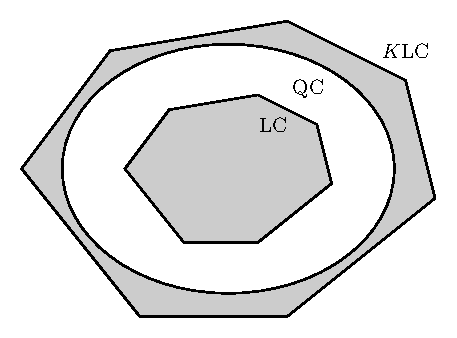
\includegraphics[scale=1]{ChapersPresentation/fig_QC&LC.pdf}
				\caption{Visualization } \label{fig:QCLC}
			\end{figure}
			
			For the implication of (2) by (1) consider figure \ref{fig:QCLC}. Since $\QC\subset K\LC$ maximizing over the elements in $K\LC$ will result in a better outcome than maximizing over the elements in $\QC$ in the direction of $M$.
		\end{proof}
	\end{frame}